% ---------------------------------------------------------------------
% Chapter: the scaling arm (Qwen2.5-7B)
% Every number is a macro from ../results/tables/numbers.tex. Do not write
% literals here -- see scripts/generate_tables.py.
% ---------------------------------------------------------------------

\chapter{Scaling the Gate: Qwen2.5-7B}
\label{ch:qwen}

\section{Why a Second Model Was Necessary}
\label{sec:qwen-why}

Every claim in Chapter~\ref{ch:eval} rests on a single quantised
Llama-3.2-3B. Two of those claims are about the \emph{mechanism} rather than
the model --- that gate thresholds must be calibrated to the model they
govern, and that retrieving selectively beats retrieving always --- and a
mechanism claim supported by one instance is an anecdote. This chapter
replicates the pipeline on Qwen2.5-7B-Instruct, roughly $2.3\times$ the
parameter count at the same \texttt{Q4\_K\_M} quantisation.

The experimental discipline is that only the model changes. The corpus is the
same MedCorp index, the questions are the same 200 MIRAGE items and the same
200 PubMedQA items, the policies are the same code paths, and the
quantisation is deliberately held at \texttt{Q4\_K\_M} so that ``larger
model'' is not confounded with ``less aggressively quantised model''. Where
something \emph{had} to change --- the gate thresholds --- that change is
itself the object of study rather than a nuisance parameter.

% AUTO-GENERATED by scripts/generate_tables.py -- DO NOT EDIT.
% Regenerate with: python scripts/generate_tables.py
% Every number is computed from results/raw_logs/ via evaluation.loading.
% git c8f491b | 2026-08-04 21:39
\begin{table}[t]
  \centering
  \begin{tabular}{llcccc}
    \toprule
    Policy & Type & $n$ & Accuracy / F1 & Retrieval & Latency/q \\
    \midrule
    \multicolumn{6}{l}{\textit{Llama-3.2-3B}} \\
    \quad P1 always-retrieve & MCQ & $200$ & 45.5\% & 100.0\% & 27\,s \\
    \quad P4 hybrid & MCQ & $200$ & 45.5\% & 100.0\% & 25\,s \\
    \quad P3 closed-book$^\dagger$ & MCQ & $200$ & 62.0\% & 0.0\% & 57\,s \\
    \quad P5 gated (calib.) & MCQ & $200$ & 54.5\% & 49.5\% & 153\,s \\
    \quad P1 always-retrieve & open & $200$ & 0.220 & 100.0\% & 23\,s \\
    \quad P3 closed-book$^\dagger$ & open & $200$ & 0.190 & 0.0\% & 27\,s \\
    \quad P5 gated (calib.) & open & $200$ & 0.211 & 79.0\% & 380\,s \\
    \midrule
    \multicolumn{6}{l}{\textit{Qwen2.5-7B}} \\
    \quad P1 always-retrieve & MCQ & $200$ & 65.0\% & 100.0\% & 5.7\,s \\
    \quad P3 closed-book$^\dagger$ & MCQ & $200$ & 74.5\% & 0.0\% & 0.1\,s \\
    \quad P5 gated (recalib.) & MCQ & $200$ & 72.0\% & 31.5\% & 300\,s \\
    \quad P1 always-retrieve & open & $200$ & 0.236 & 100.0\% & 8.0\,s \\
    \quad P3 closed-book$^\dagger$ & open & $200$ & 0.256 & 0.0\% & 2.3\,s \\
    \quad P5 gated (recalib.) & open & $200$ & 0.248 & 43.5\% & 24\,s \\
    \midrule
    \multicolumn{6}{l}{\textit{Qwen2.5-14B}} \\
    \quad P1 always-retrieve & MCQ & $200$ & 53.0\% & 100.0\% & 8.7\,s \\
    \quad P3 closed-book$^\dagger$ & MCQ & $200$ & 75.5\% & 0.0\% & 0.3\,s \\
    \quad P5 gated (recalib.) & MCQ & $200$ & 68.5\% & 24.0\% & 15\,s \\
    \quad P1 always-retrieve & open & $200$ & 0.245 & 100.0\% & 10\,s \\
    \quad P3 closed-book$^\dagger$ & open & $200$ & 0.255 & 0.0\% & 5.4\,s \\
    \quad P5 gated (recalib.) & open & $200$ & 0.249 & 51.5\% & 32\,s \\
    \bottomrule
  \end{tabular}
  \caption{The scaling arm. Identical corpus, identical questions and identical
  policy definitions across both models, so a difference is attributable to model
  scale. Multiple-choice is scored by accuracy, open-ended by mean token-F1.
  $^{\dagger}$P3 never retrieves and is corpus-independent. The Qwen open-ended
  P5 row uses thresholds refitted for open-ended drafts (a single global operating
  point per task type); reusing the multiple-choice thresholds instead saturates the
  gate (Table~\ref{tab:gate-saturation}). Retrieval budgets are \emph{not}
  matched across models; see Table~\ref{tab:budget-match}.}
  \label{tab:scaling-results}
\end{table}


\section{Closed-Book Capability Rises With Scale}
\label{sec:qwen-closedbook}

Closed-book accuracy rises from \accPthreeMcq{} to \accQwenPthreeMcq{}, an
unpaired difference of \diffQwenLlamaMcq{}pp with a 95\% interval of
\diffQwenLlamaMcqCI{}. Because both models answered the identical question
set, the paired comparison is the more informative one: of \mcnemarN{}
questions, \mcnemarBoth{} were answered correctly by both models,
\mcnemarNeither{} by neither, \mcnemarOnlyQwen{} by Qwen alone and
\mcnemarOnlyLlama{} by Llama alone. McNemar's test on the discordant pairs
gives $\chi^2 = \mcnemarChi{}$, comfortably beyond the $3.84$ threshold for
$p < 0.05$. The larger model is genuinely better at this benchmark, and the
$\mcnemarOnlyLlama{}$ questions it loses show the gain is not simply
additive.

This matters for the thesis in an uncomfortable way. The project's argument
for retrieval rests partly on small models lacking parametric medical
knowledge; a model that answers three quarters of MMLU-Med from memory needs
retrieval less often, not more. Section~\ref{sec:qwen-budget} shows that the
gate does in fact retrieve less on Qwen --- but for reasons that turn out to
be only partly the intended ones.

\section{Calibration Does Not Transfer --- Confirmed Prospectively}
\label{sec:qwen-nontransfer}

The single-model version of this claim (Section~\ref{sec:eval-calibration})
was necessarily retrospective: thresholds were found not to fire, and were
then refitted. On Qwen the claim was tested \emph{before} the evaluation ran.
Applying the 3B's shipped $\tau = 0.70/0.70$ to a 50-question calibration
sample of Qwen produced an ensemble retrieval rate of
\retQwenCalibAtLlamaTau{}: the operating point was almost entirely
degenerate, and P5 would have been indistinguishable from closed-book P3.

This is the strongest available form of the claim. The prediction was made
from the 3B's signal distribution, the test was run on a model that did not
exist in the original experiment, and the predicted failure occurred. Gate
thresholds are properties of a model's signal distribution, not constants of
the method.

Thresholds were therefore refitted by matching the 3B's \emph{per-gate
retrieval budget} rather than by copying its $\tau$. Copying $\tau$ preserves
a number that means nothing across models; matching the budget preserves the
quantity the comparison is actually about, since ``selective beats
always-retrieve'' is a claim about accuracy \emph{at a given retrieval rate}.

\section{The Budget Did Not Match, and Why}
\label{sec:qwen-budget}

% AUTO-GENERATED by scripts/generate_tables.py -- DO NOT EDIT.
% Regenerate with: python scripts/generate_tables.py
% Every number is computed from results/raw_logs/ via evaluation.loading.
% git 855a45b | 2026-08-02 01:10
\begin{table}[t]
  \centering
  \begin{tabular}{llcccc}
    \toprule
    & & \multicolumn{3}{c}{per-member vote rate} & \\
    \cmidrule(lr){3-5}
    Model & Task & entropy & margin & probe & ensemble \\
    \midrule
    Llama-3.2-3B & MCQ & 52.0\% & 53.5\% & 40.0\% & 49.5\% \\
    Llama-3.2-3B & open & 75.5\% & 79.0\% & 87.0\% & 79.0\% \\
    Qwen2.5-7B & MCQ & 34.5\% & 40.5\% & 7.5\% & 31.5\% \\
    Qwen2.5-7B & open (MCQ $\tau$) & 100.0\% & 100.0\% & 82.9\% & 100.0\% \\
    Qwen2.5-7B & open (recalib.) & 47.0\% & 39.5\% & 47.5\% & 43.5\% \\
    Qwen2.5-14B & MCQ & 29.5\% & 29.0\% & 7.5\% & 24.0\% \\
    Qwen2.5-14B & open & 46.0\% & 43.5\% & 63.5\% & 51.5\% \\
    \bottomrule
  \end{tabular}
  \caption{Realised retrieval budgets. Thresholds for Qwen were refitted to
  reproduce the 3B's per-gate budget, and the two tunable members landed close to
  target. The probe could not follow: on multiple-choice it is threshold-free
  (two drafts agree or they do not), so it cannot be recalibrated, and the larger
  model self-agrees far more often. With one member near-silent, a
  majority-of-three vote cannot reach the intended rate. The consequence is that
  the two models operate at different budgets, so ``selective retrieval beats
  always-retrieve at a matched budget'' is established \emph{within} each model
  but not \emph{across} them.}
  \label{tab:budget-match}
\end{table}


The refit did not achieve its target. Against the 3B's \retPfiveMcq{}
ensemble budget, Qwen realised \retQwenPfiveMcq{}. The two tunable members
landed close to target; the failure is entirely attributable to the third.

On multiple-choice the hallucination probe is threshold-free by construction:
it generates two differently-framed drafts and votes to retrieve when the
extracted answer letters disagree. There is no parameter to move. Its vote
rate fell from \probeFireLlamaMcq{} on Llama to \probeFireQwenMcq{} on Qwen,
because the larger model simply agrees with itself far more often across
framings. With one member of a majority-of-three vote effectively silent, the
ensemble reduces to ``entropy \emph{and} margin'' --- a conjunction, and a
strictly harder condition than the majority rule it replaces --- so the
achievable budget falls below target no matter how the other two are tuned.

This is a genuine finding about gate ensembles at scale rather than a
misconfiguration, and it has a design implication: an ensemble whose members
are not all recalibratable cannot hold a retrieval budget constant across
models. It is also, unavoidably, a limitation on the cross-model comparison,
and it is recorded as one in Section~\ref{sec:disc-limitations}.

\begin{figure}[t]
  \centering
  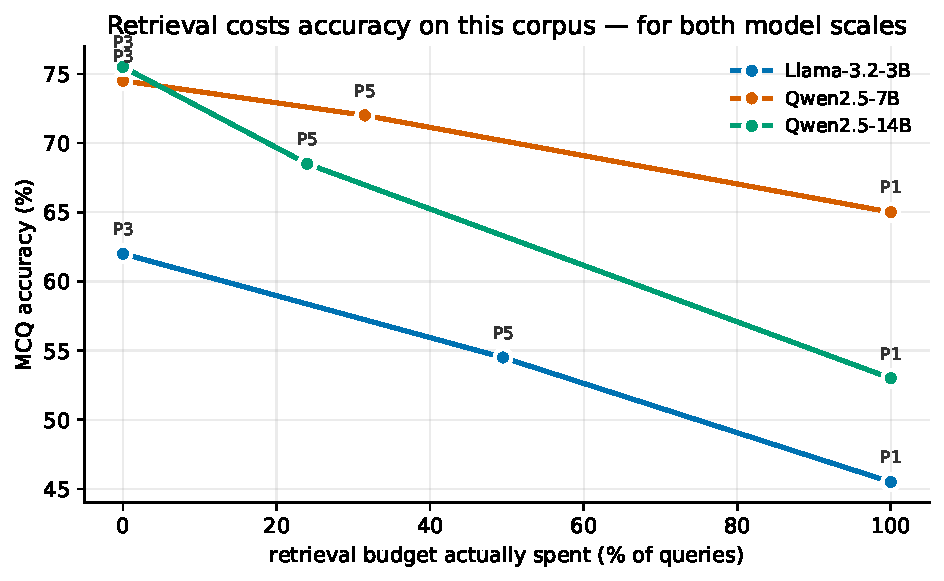
\includegraphics[width=0.8\linewidth]{results/figures/fig_scaling}
  \caption{Multiple-choice accuracy against the retrieval budget actually
    spent. Both models lose accuracy as retrieval increases on this corpus,
    and Qwen sits uniformly higher. The two P5 points do not share an
    $x$-position: the budgets are not matched, which is precisely the
    limitation discussed in Section~\ref{sec:qwen-budget}.}
  \label{fig:scaling}
\end{figure}

\section{Gate Saturation on Open-Ended Questions}
\label{sec:qwen-saturation}

The thresholds refitted in Section~\ref{sec:qwen-nontransfer} were fitted on
multiple-choice drafts and then reused, unchanged, for the open-ended runs.
That reuse is unsound, and the open-ended evidence shows how badly.

% AUTO-GENERATED by scripts/generate_tables.py -- DO NOT EDIT.
% Regenerate with: python scripts/generate_tables.py
% Every number is computed from results/raw_logs/ via evaluation.loading.
% git 855a45b | 2026-08-02 01:10
\begin{table}[t]
  \centering
  \small
  \begin{tabular}{lllcc}
    \toprule
    Model / task & Gate & $\tau$ & signal min / med / max & fires \\
    \midrule
    Llama-3.2-3B / MCQ & entropy & 0.700 & 0.200 / 0.718 / 1.532 & 52.0\% \\
     & margin & 0.700 & 0.462 / 0.695 / 0.892 & 53.5\% \\
     & probe & --- & --- (threshold-free) & 40.0\% \\
    \midrule
    Llama-3.2-3B / open & entropy & 0.700 & 0.324 / 0.877 / 1.744 & 75.5\% \\
     & margin & 0.700 & 0.346 / 0.624 / 0.853 & 79.0\% \\
     & probe & 0.700 & 0.071 / 0.509 / 1.000 & 87.0\% \\
    \midrule
    Qwen2.5-7B / MCQ & entropy & 0.187 & 0.000 / 0.241 / 0.960 & 34.5\% \\
     & margin & 0.899 & 0.712 / 0.927 / 1.000 & 40.5\% \\
     & probe & --- & --- (threshold-free) & 7.5\% \\
    \midrule
    Qwen2.5-7B / open (MCQ $\tau$) & entropy & 0.187 & 0.215 / 0.540 / 1.001 & \textbf{100.0\%} \\
     & margin & 0.899 & 0.658 / 0.769 / 0.854 & \textbf{100.0\%} \\
     & probe & 0.700 & 0.077 / 0.538 / 0.836 & 82.9\% \\
    \midrule
    Qwen2.5-7B / open (recalib.) & entropy & 0.568 & 0.050 / 0.554 / 1.119 & 47.0\% \\
     & margin & 0.752 & 0.618 / 0.766 / 0.972 & 39.5\% \\
     & probe & 0.538 & 0.053 / 0.545 / 1.000 & 47.5\% \\
    \midrule
    Qwen2.5-14B / MCQ & entropy & 0.250 & 0.000 / 0.324 / 0.791 & 29.5\% \\
     & margin & 0.861 & 0.551 / 0.921 / 0.999 & 29.0\% \\
     & probe & --- & --- (threshold-free) & 7.5\% \\
    \midrule
    Qwen2.5-14B / open & entropy & 0.536 & 0.138 / 0.514 / 0.929 & 46.0\% \\
     & margin & 0.750 & 0.609 / 0.760 / 0.922 & 43.5\% \\
     & probe & 0.712 & 0.250 / 0.643 / 1.000 & 63.5\% \\
    \bottomrule
  \end{tabular}
  \caption{Gate saturation. The entropy gate fires when its signal exceeds
  $\tau$; the margin and probe gates fire when theirs fall below it. For
  Qwen on open-ended questions the entropy signal's \emph{minimum} lies above
  its threshold and the margin signal's \emph{maximum} lies below its own, so
  every question retrieves and P5 degenerates into P1. Both thresholds were fitted
  on multiple-choice drafts and reused unchanged on open-ended drafts, whose signal
  distributions differ; the probe is threshold-free on MCQ (letter agreement) and
  so reports no range there. Llama saturates less only because its $\tau=0.70$
  happens to fall inside its open-ended distribution.}
  \label{tab:gate-saturation}
\end{table}


The entropy gate votes to retrieve when its signal exceeds $\tau$. On Qwen's
open-ended questions the \emph{smallest} observed signal,
\qwenOpenEntropyMin{}, already exceeds its threshold of
\qwenOpenEntropyTau{}. The margin gate votes when its signal falls below
$\tau$; its \emph{largest} observed signal, \qwenOpenMarginMax{}, lies below
its threshold of \qwenOpenMarginTau{}. Neither gate has a decision to make.
Every question retrieved, the ensemble rate was \retQwenPfiveOpen{}, and P5
on open-ended questions is not a selective policy at all --- it is P1 wearing
P5's name. No selective-retrieval claim can be drawn from that run.

\begin{figure}[t]
  \centering
  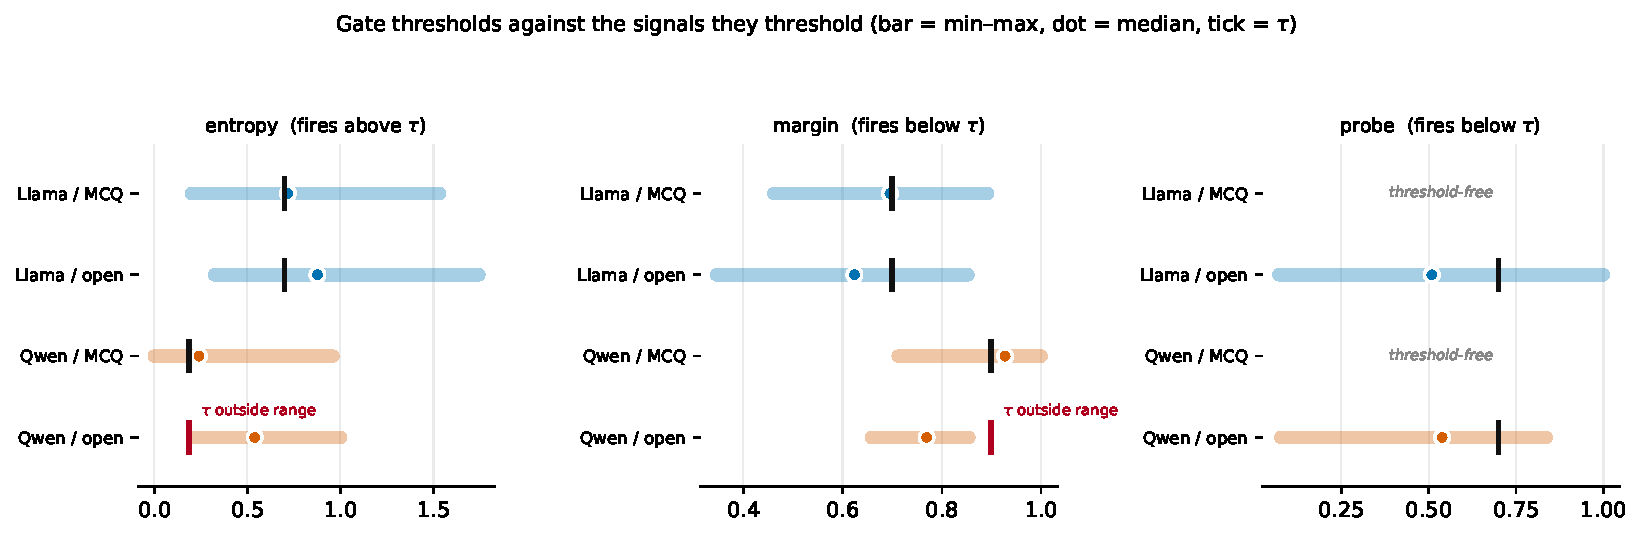
\includegraphics[width=\linewidth]{results/figures/fig_gate_saturation}
  \caption{Each gate's threshold against the distribution of the signal it
    thresholds. A threshold drawn outside its own range bar is a gate with no
    decision to make. Both of Qwen's logit gates are in that state on
    open-ended questions.}
  \label{fig:gate-saturation}
\end{figure}

The cause is a distributional shift the method did not anticipate. A
multiple-choice draft is a single letter; an open-ended draft is a paragraph
of free text. There is no reason for the per-token entropy or the top-two
probability margin of those two generations to occupy the same range, and
they do not (Figure~\ref{fig:signal-shift}). The lesson generalises beyond
this model: \textbf{gate thresholds are task-specific, not merely
model-specific}, and a threshold fitted on one question format must not be
deployed on another.

Llama escapes total saturation on the same task only by luck. Its
$\tau = 0.70$, fitted on its own multiple-choice signals, happens to fall
inside its open-ended distribution, so its gates still discriminate --- at a
retrieval rate of \retPfiveOpen{}, far above the intended budget, but not at
the degenerate ceiling.

\begin{figure}[t]
  \centering
  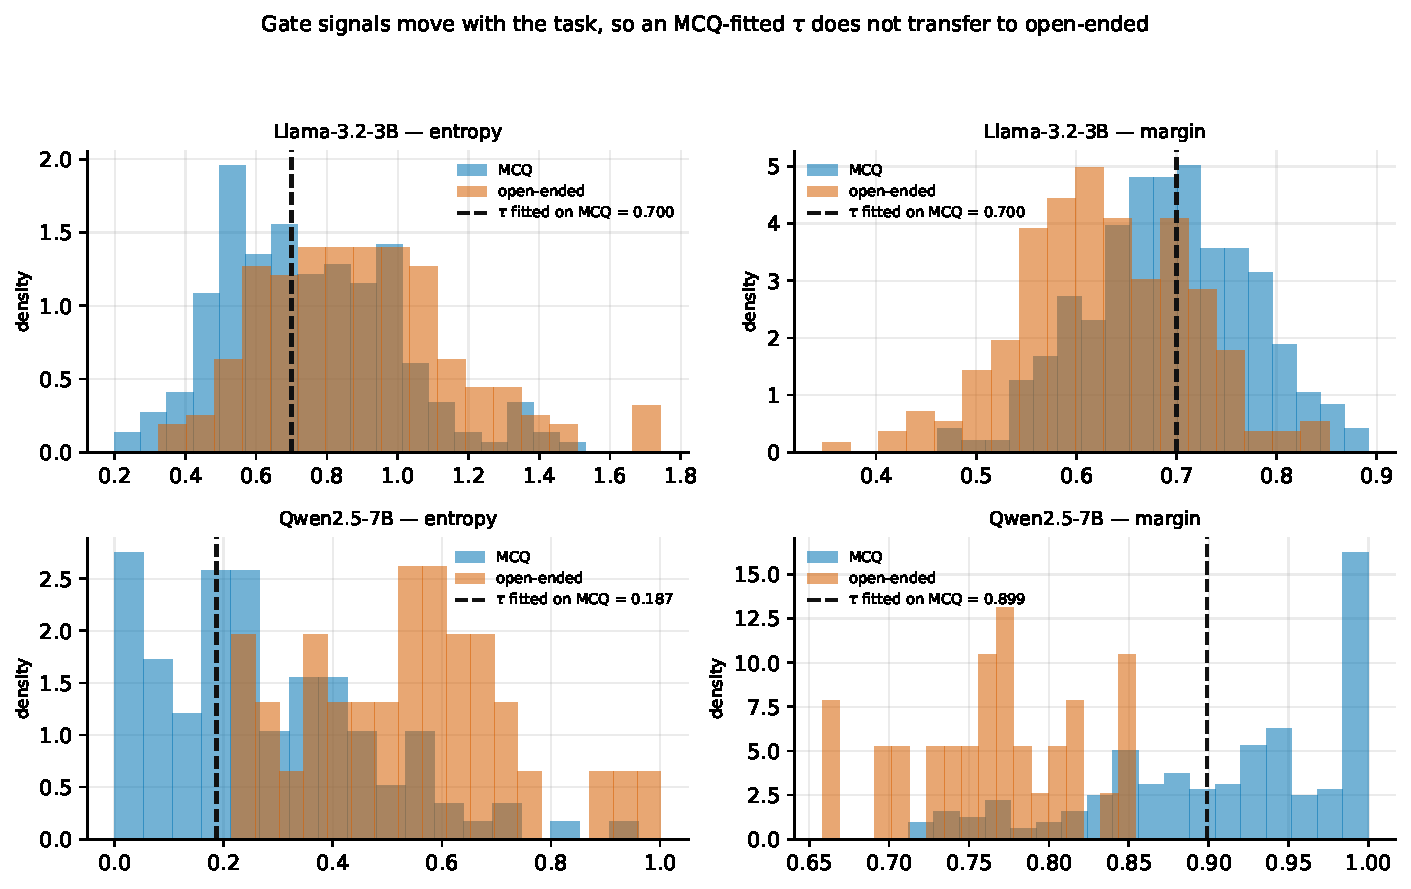
\includegraphics[width=\linewidth]{results/figures/fig_signal_shift}
  \caption{Gate-signal distributions for the same model and the same gate on
    multiple-choice versus open-ended questions, with the multiple-choice
    threshold overlaid. The distributions barely overlap, which is why a
    threshold fitted on one lands in the wrong part of the other.}
  \label{fig:signal-shift}
\end{figure}

\section{Open-Ended Results}
\label{sec:qwen-open}

Qwen's closed-book open-ended score is \fOneQwenPthreeOpen{} mean token-$F_1$
over the full 200 questions, against \fOnePthreeOpen{} for Llama --- the same
substantial lift with scale seen on multiple-choice. The gated policy, run with
thresholds refitted for open-ended drafts (the multiple-choice thresholds
saturate the gate here, Section~\ref{sec:qwen-saturation}), scores
\fOneQwenPfiveOpen{} at \retQwenPfiveOpen{} retrieval, also over the full 200
questions. The open-ended arm is therefore measured at full sample for every
policy on both models.

The three policies fall in the order P3 $>$ P5 $>$ P1
(\fOneQwenPthreeOpen{} $>$ \fOneQwenPfiveOpen{} $>$ \fOneQwenPoneOpen{}):
closed-book is best and each additional unit of retrieval costs accuracy,
exactly as on multiple-choice. This is the reverse of the smaller model, where
open-ended retrieval \emph{helped} (P1 \fOnePoneOpen{} $>$ P5 \fOnePfiveOpen{}
$>$ P3 \fOnePthreeOpen{}). The cross-model reversal --- and what it says about
when retrieval is worth its cost --- is taken up in
Section~\ref{sec:cmp-open}; here it is enough to record that scaling moves the
open-ended arm in the same direction as multiple-choice, so ``retrieval hurts on
this corpus'' is not confined to one task type at the larger scale.

Two caveats travel with these numbers. The gated budgets are not matched across
models (\retQwenPfiveOpen{} against \retPfiveOpen{}), so the P5 rows are read as
positions within each model's own P1--P3 range rather than as a matched-budget
comparison. And paragraph-level token-$F_1$ is surface-lexical and low in
absolute terms for both models, so only the ordering is interpreted, never the
magnitude of a gap.

\section{What the Scaling Arm Establishes}
\label{sec:qwen-summary}

Four things survive scrutiny. Closed-book capability rises substantially
with scale, and the paired test supports that at $p < 0.05$. Calibration
non-transfer was confirmed prospectively on a model the original experiment
never saw, which is the strongest form the claim can take in this project.
The ordering P3 $>$ P5 $>$ P1 holds on multiple-choice at both scales, so
``retrieval hurts on this corpus, and gating limits the damage'' is no longer a
single-model observation. And the open-ended arm, measured at full sample on
both models, reverses its policy ordering between scales
(Section~\ref{sec:cmp-open}): retrieval that helped the smaller model
harms the larger one, which localises the value of retrieval to the gap between
what a model already knows and what the corpus adds.

One thing does not survive. The cross-model retrieval budgets differ by
\budgetGapMcq{} percentage points, because the threshold-free probe could not be
recalibrated once the larger model began agreeing with itself
(Section~\ref{sec:qwen-budget}). Accuracy-at-matched-budget is therefore
established within each model but not across them, and the cross-model claims
rest on the budget-independent comparisons --- closed-book accuracy and the
direction of each policy ordering --- rather than on the gated rows directly.
